%%%%%%%%%%%%%%%%%%%%%%%%%%%%%%%%%%%%%%%%%
% MHL Thesis LaTeX Template
% Version 1.1 (09/09/2021)
%
% This template is based on a template by:
% Steve Gunn (http://users.ecs.soton.ac.uk/srg/softwaretools/document/templates/)
% Sunil Patel (http://www.sunilpatel.co.uk/thesis-template/)
%
% found on:
% http://www.LaTeXTemplates.com/template/masters-doctoral-thesis
%
% Template license:
% CC BY-NC-SA 3.0 (http://creativecommons.org/licenses/by-nc-sa/3.0/)
%%%%%%%%%%%%%%%%%%%%%%%%%%%%%%%%%%%%%%%%%

%----------------------------------------------------------------------------------------
%	DOCUMENT CONFIGURATIONS
%----------------------------------------------------------------------------------------
\PassOptionsToPackage{greek,main=english}{babel}
\documentclass[
	12pt, % The default document font size, options: 10pt, 11pt, 12pt
	% oneside, % Two side (alternating margins) for binding by default, uncomment to switch to one side
	english,
	onehalfspacing, % Single line spacing, alternatives: singlespacing or doublespacing
	%draft, % Uncomment to enable draft mode (no pictures, no links, overfull hboxes indicated)
	%nolistspacing, % If the document is onehalfspacing or doublespacing, uncomment this to set spacing in lists to single
	liststotoc, % Uncomment to add the list of figures/tables/etc to the table of contents
	toctotoc, % Uncomment to add the main table of contents to the table of contents
	parskip, % Uncomment to add space between paragraphs
	%nohyperref, % Uncomment to not load the hyperref package
	headsepline, % Uncomment to get a line under the header
	% chapterinoneline, % Uncomment to place the chapter title next to the number on one line
	% consistentlayout, % Uncomment to change the layout of the declaration, abstract and acknowledgements pages to match the default layout
]{MastersDoctoralThesis} % The class file specifying the document structure

%----------------------------------------------------------------------------------------
%	PACKAGES
%----------------------------------------------------------------------------------------

\usepackage[utf8]{inputenc} % Required for inputting international characters
\usepackage[LGR, T1]{fontenc} % Output font encoding for international characters
\usepackage{mathpazo} % Use the Palatino font by default
\usepackage[backend=biber,style=numeric,natbib=true,sorting=none]{biblatex} % Use the bibtex backend with the numeric citation style
\usepackage[autostyle=true]{csquotes} % Required to generate language-dependent quotes in the bibliography
\usepackage[section]{placeins}
\usepackage{float}
\usepackage{comment}
\usepackage{algorithm}
\usepackage[noend]{algpseudocode}
\usepackage{hyperref}
\usepackage{graphicx}
\usepackage{amsmath}

\makeatletter
\makeatother
\def\infinity{\rotatebox{90}{8}}
\addtocontents{loa}{\def\string\figurename{Algorithm}}

%----------------------------------------------------------------------------------------
%	BIBLIOGRAPHY FILES
%----------------------------------------------------------------------------------------

% Todo: comment out example.bib file when done reading the template instructions
% \addbibresource{example.bib} % The filename of the bibliography
\addbibresource{references.bib} % The filename of the bibliography

%----------------------------------------------------------------------------------------
%	MARGIN SETTINGS
%----------------------------------------------------------------------------------------

\geometry{
	paper=a4paper, % Change to letterpaper for US letter
	inner=2.5cm, % Inner margin
	outer=3.8cm, % Outer margin
	bindingoffset=.5cm, % Binding offset
	top=1.5cm, % Top margin
	bottom=1.5cm, % Bottom margin
	%showframe, % Uncomment to show how the type block is set on the page
}

%----------------------------------------------------------------------------------------
%	THESIS INFORMATION
%----------------------------------------------------------------------------------------

% Todo: fill info below
\thesistitle{Interactive User Environment Application on Kubernetes} % Your thesis title, this is used in the title and abstract, print it elsewhere with \ttitle
\author{Kyriakos \textsc{Chalvatzis}} % Your name, this is used in the title page and abstract, print it elsewhere with \authorname
\supervisor{Prof.Vasilis \textsc{Samoladas}} % Your supervisor's name, this is used in the title page, print it elsewhere with \supname
\degree{Electrical and Computer Engineer} % Your degree name, this is used in the title page and abstract, print it elsewhere with \degreename
\subject{Electrical and Computer Engineering} % Your subject area, this is not currently used anywhere in the template, print it elsewhere with \subjectname
\keywords{Diploma Thesis} % Keywords for your thesis, this is not currently used anywhere in the template, print it elsewhere with \keywordnames
\university{\href{https://www.tuc.gr/}{Technical University of Crete}} % Your university's name and URL, this is used in the title page and abstract, print it elsewhere with \univname
\department{\href{https://www.ece.tuc.gr/}{School of Electrical and Computer Engineering}} % Your department's name and URL, this is used in the title page and abstract, print it elsewhere with \deptname
% \group{\href{https://www.mhl.tuc.gr/}{Microprocessor and Hardware Laboratory}} % Your research group's name and URL, this is used in the title page, print it elsewhere with \groupname
\faculty{
		% \href{http://faculty.university.com}{Faculty Name}
} % Your faculty's name and URL, this is used in the title page and abstract, print it elsewhere with \facname

\AtBeginDocument{
	\hypersetup{pdftitle=\ttitle} % Set the PDF's title to your title
	\hypersetup{pdfauthor=\authorname} % Set the PDF's author to your name
	\hypersetup{pdfkeywords=\keywordnames} % Set the PDF's keywords to your keywords
}

%----------------------------------------------------------------------------------------
%	TITLE PAGE
%----------------------------------------------------------------------------------------

\begin{document}

\frontmatter % Use roman page numbering style (i, ii, iii, iv...) for the pre-content pages

\pagestyle{plain} % Default to the plain heading style until the thesis style is called for the body content

\begin{titlepage}
	\begin{center}
		{\scshape\LARGE \univname\par}
		\vspace{0.5cm} % University name
		\textsc{\Large Diploma Thesis}\\[0.5cm] % Thesis type

		\HRule\\[0.4cm] % Horizontal line
		{\huge \bfseries \ttitle\par}\vspace{0.4cm} % Thesis title

		\begin{minipage}[t]{0.4\textwidth}
			\begin{flushleft} \large
				\emph{Author:}\\
				% Todo: fill correct link
				\href{http://example.com/}{\authorname} % Author name - remove the \href bracket to remove the link
			\end{flushleft}
		\end{minipage}
		\begin{minipage}[t]{0.5\textwidth}
			\begin{flushright} \large
				\emph{Thesis Committee:} \\
				% Todo: fill correct link
				\href{https://www.ece.tuc.gr/el/index.php?id=4109&tx_tuclabspersonnel_list%5Bperson%5D=361&tx_tuclabspersonnel_list%5Baction%5D=person&tx_tuclabspersonnel_list%5Bcontroller%5D=List}{\supname}\\ % Supervisor name - remove the \href bracket to remove the link
				% Todo: fill correct link, full name
				\href{https://www.ece.tuc.gr/el/i-scholi/prosopiko/single-display-person?tx_tuclabspersonnel_pi3%5Bpersonid%5D=771&cHash=7632eaf07b3963f9d990de818bdbcda9}{Prof. Name \textsc{Giatrakos}}\\
				% Todo: fill correct link, full name
				\href{https://www.ece.tuc.gr/el/index.php?id=4109&tx_tuclabspersonnel_list%5Bperson%5D=353&tx_tuclabspersonnel_list%5Baction%5D=person&tx_tuclabspersonnel_list%5Bcontroller%5D=List}{Prof. Name \textsc{Petrakis}}
			\end{flushright}
		\end{minipage}\\[0.2cm]

		
\includegraphics[scale=0.21]{Images/TUC_logo.png} % University/department logo - uncomment to place it
		\\
		
		\vfill

		\large \textit{A thesis submitted in fulfillment of the requirements\\ for the diploma of \degreename}\\[0.3cm] % University requirement text
		\textit{in the}\\[0.4cm]
		% \deptname\\\groupname\\[2cm] % Research group name and department name
		\deptname\\[2cm] % Research group name and department name

		\vfill

		{\large \today}\\ % Date
		\vfill
	\end{center}
\end{titlepage}

%----------------------------------------------------------------------------------------
%	ABSTRACT PAGE English
%----------------------------------------------------------------------------------------

\begin{abstract}
	\addchaptertocentry{\abstractname} % Add the abstract to the table of contents
	% Todo: Add English Abstract
	The Thesis Abstract is written here (and usually kept to just this page). The page is kept centered vertically so can expand into the blank space above the title too\ldots
\end{abstract}

%----------------------------------------------------------------------------------------
%	ABSTRACT PAGE Greek
%----------------------------------------------------------------------------------------

\begin{abstract}
	\addchaptertocentry{\abstractname} % Add the abstract to the table of contents
	% Todo: Add Greek Abstract
    \selectlanguage{greek}
	Η περίληψη της διπλωματικής γράφεται εδώ (και συνήθως αποτελεί αυτή την μία μόνο σελίδα). Η σελίδα αυτή κρατάται στοιχισμένη στην μέση οριζόντια και κάθετα, ώστε να μπορεί να επεκτίνεται στον κενό χώρο και πάνω από τον τίτλο\ldots
	
\end{abstract}

%----------------------------------------------------------------------------------------
%	ACKNOWLEDGEMENTS
%----------------------------------------------------------------------------------------

\begin{acknowledgements}
	\addchaptertocentry{\acknowledgementname} % Add the acknowledgements to the table of contents
	% Todo: Add Acknowledgements
	The acknowledgments and the people to thank go here, don't forget to include your project advisor\ldots
\end{acknowledgements}

%----------------------------------------------------------------------------------------
%	LIST OF CONTENTS/FIGURES/TABLES PAGES
%----------------------------------------------------------------------------------------

\tableofcontents % Prints the main table of contents
\listoffigures % Prints the list of figures
\listoftables % Prints the list of tables
\listofalgorithms% Prints the list of algorithms
\addcontentsline{toc}{chapter}{List of Algorithms}

%----------------------------------------------------------------------------------------
%	ABBREVIATIONS
%----------------------------------------------------------------------------------------

% Todo: edit to your requirements
% spell-checker: disable
\begin{abbreviations}{ll} % Include a list of abbreviations (a table of two columns)]
	\textbf{ALU}	& \textbf{A}rithmetic \textbf{L}ogic \textbf{U}nit\\
	\textbf{ASIC}	& \textbf{A}pplication \textbf{S}pecific \textbf{I}ntegrated \textbf{C}ircuit\\
	\textbf{BRAM}	& \textbf{B}lock \textbf{R}andom \textbf{A}ccess \textbf{M}emory\\
	\textbf{CPU}	& \textbf{C}entral \textbf{P}rocessor \textbf{U}nit\\
	\textbf{CS}		& \textbf{C}omputer \textbf{S}cience\\
	\textbf{DDR4}	& \textbf{D}ouble \textbf{D}ata \textbf{R}ate type \textbf{4} memory\\
	\textbf{DRAM}	& \textbf{D}ynamic \textbf{R}andom \textbf{A}ccess \textbf{M}emory\\
	\textbf{DSP}	& \textbf{D}igital \textbf{S}ignal \textbf{P}rocessor\\
	\textbf{FF}		& \textbf{F}lip \textbf{F}lops\\
	\textbf{FPGA}	& \textbf{F}ield \textbf{P}rogrammable \textbf{G}ate \textbf{A}rray\\
	\textbf{GDDR6}	& \textbf{G}raphics \textbf{D}ouble \textbf{D}ata \textbf{R}ate type \textbf{6} memory\\
	\textbf{GPU}	& \textbf{G}raphic \textbf{P}rocessor \textbf{U}nit\\
	\textbf{HBM}	& \textbf{H}igh \textbf{B}andwidth \textbf{M}emory\\
	\textbf{HDL}	& \textbf{H}ardware \textbf{D}escription \textbf{L}anguage\\
	\textbf{HLS}	& \textbf{H}igh \textbf{L}evel \textbf{S}ynthesis\\
	\textbf{HPC}	& \textbf{H}ight \textbf{P}erformance \textbf{C}omputing\\
	\textbf{LUT}	& \textbf{L}ook \textbf{U}p \textbf{T}able\\
	\textbf{MPSoC}	& \textbf{M}ulti \textbf{P}rocessor \textbf{S}ystem \textbf{o}n \textbf{C}hip\\
	\textbf{PL}		& \textbf{P}rogrammable \textbf{L}ogic\\
	\textbf{PS}		& \textbf{P}rocessing \textbf{S}ystem\\
	\textbf{RAM}	& \textbf{R}andom \textbf{A}ccess \textbf{M}emory\\
	\textbf{SDK}	& \textbf{S}oftware \textbf{D}evelopment \textbf{K}it\\
	\textbf{SIMD}	& \textbf{S}ingle \textbf{I}nstruction \textbf{M}ultiple \textbf{D}ata\\
	\textbf{SSE}	& \textbf{S}treaming \textbf{S}IMD \textbf{E}xtensions\\
	\textbf{SSD}	& \textbf{S}olid \textbf{S}tate \textbf{D}rive\\
	\textbf{TDP}	& \textbf{T}hermal \textbf{D}esign \textbf{P}ower\\
	\textbf{URAM}	& \textbf{U}ltra \textbf{R}andom \textbf{A}ccess \textbf{M}emory\\
	\textbf{USD}	& \textbf{U}nited \textbf{S}tates \textbf{D}ollar\\
\end{abbreviations}
% spell-checker: enable

%----------------------------------------------------------------------------------------
%	DEDICATION
%----------------------------------------------------------------------------------------

\dedicatory{Dedicated to my family and friends\ldots}

%----------------------------------------------------------------------------------------
%	THESIS CONTENT - CHAPTERS
%----------------------------------------------------------------------------------------

% Include the chapters of the thesis as separate files from the Chapters folder
% Uncomment the lines as you write the chapters
\pagestyle{thesis} % Return the page headers back to the "thesis" style
\mainmatter% Begin numeric (1,2,3...) page numbering

\chapter{Introduction}
\label{Chapter-Introduction}

\section{Purpose and Motivation}
\hspace{2mm}This project began as an effort to integrate a user-friendly `environment' layer into Kubernetes—an infrastructure known 
for its power and scalability, yet lacking direct support for user-centric entities. The goal was to make 
an environment where individual users can perform analytical computing in their own `space', especially enabling
data analysts to work with large-scale datasets, by abstracting the complexity of orchestration and container management.
As the system evolved, the focus deviated slightly towards a fully modular full stack platform that supports multiple users, secures
access with custom authentication, and enables storage provisioning, sharing, and execution of batch jobs using familiar tools such
as DuckDB, Bash, Octave, and Pandas~\cite{mckinney-proc-scipy-2010}. The motivation became to deliver a system 
that combines the robustness of cloud-native
technologies with the ease of use of desktop analytical environments—bridging the gap between DevOps infrastructure and 
end-user data workflows.

Ultimately, amongst some services, the bar was set to implement already existing enterprise level technology stacks to 
more basic and developer friendly as in ease of access and deployment versions. It had been a personal aspiration and 
challenge to create some utilities that are scoped for development with a laconic tone while maintaining inspiration by others.

\newpage

\section{Problem Statement}

\hspace{2mm}While modern data platforms such as Apache Airflow or Spark 
address large-scale, enterprise-level orchestration needs, they are often complex, heavyweight, and 
not designed with ease of use or modularity in mind—especially for individual analysts or smaller 
teams working on self-contained workflows.

This thesis does not seek to compete with such platforms, nor to introduce fundamentally new orchestration paradigms. 
Instead, it focuses on designing and implementing a lightweight, extensible system that simplifies the execution of batch 
data analysis jobs in a multi-user environment.

The core problem addressed is the absence of a simple, user-accessible platform where authenticated users can:
\begin{itemize}
    \item Upload datasets to a common, structured storage layer,
    \item Submit analytical jobs using containerized tools such as DuckDB, Pandas, or Octave,
    \item View job outputs and logs through a unified interface,
    \item And share or manage their data and jobs in a collaborative way.
\end{itemize}

This project presents a custom application built on top of Kubernetes~\cite{google-kubernetes} that abstracts away infrastructure complexity, 
offering a modular foundation upon which analytical tools can be plugged and executed in a reproducible, isolated manner. 
The overarching goal is to improve the user experience in running batch data workflows—not by reimagining distributed computation, 
but by making its power more accessible and flexible for real-world analysis tasks.



\section{Scope of the Project}
\hspace{2mm}The scope of this thesis includes the design, development, and integration of a modular microservice-based platform tailored to Kubernetes. 
The system introduces:

\begin{itemize}
    \item A custom authentication and user management service (\texttt{Minioth}).
    \item A central orchestration service (\texttt{Uspace}) that defines and manages user environments.
    \item A lightweight virtual filesystem abstraction (\texttt{Fslite}) for managing user data and metadata.
    \item Integration with MinIO for physical object storage.
    \item A WebSocket-enabled frontend service that provides real-time interaction and job monitoring capabilities.
\end{itemize}

The system supports uploading, sharing, and executing batch jobs using containerized tools, while abstracting the complexity of 
Kubernetes operations from the end user.

Out of scope for this project are scheduling algorithms, dynamic autoscaling and support for third-party 
authentication (e.g., OAuth~\cite{oauth2-rfc6749}).

The system is implemented in Go~\cite{golang}, a statically typed, compiled programming language designed for simplicity and concurrency.

The backend for the Services is implemented using the Gin web framework for Go~\cite{gingonic}, which provides performant HTTP routing and middleware integration.

\section{Thesis Contributions}
\hspace{2mm}The primary contributions of this thesis are as follows:
\begin{itemize}
    \item The design and implementation of a fully functional user-centric platform deployed on Kubernetes, 
    abstracting core orchestration mechanics from the user.
    \item A custom authentication service (\texttt{Minioth}) implementing user/group-based access control with secure 
    token issuance and verification.
    \item The \texttt{Uspace} service that defines and manages user environments, enabling secure job submission and resource 
    isolation.
    \item The \texttt{Fslite} abstraction layer that models user data and virtual resources in a hierarchical structure, 
    backed by object storage (MinIO).
    \item A WebSocket-integrated frontend allowing users to interactively monitor jobs and access 
    their workspace in real time.
    \item A demonstration of how Kubernetes-native resources and batch execution can be adapted to serve multi-user analytical 
    workflows in an accessible, extensible system.
\end{itemize}



\newpage
\section{Thesis Outline}
% Todo: Fill chapter descriptions
\begin{itemize}
    \item \textbf{Chapter 2 – Background and Theoretical Foundations:}  
    An overview of the core technologies and concepts underpinning the system, including Kubernetes, microservices, authentication models, 
    containerized workloads, and object storage.

    \item \textbf{Chapter 3 – Related Work:}  
    A review of existing platforms and tools related to data processing, user environment provisioning, and cloud-native architectures. 
    It highlights their limitations and positions this work within the broader landscape.

    \item \textbf{Chapter 4 – System Design and Architecture:}  
    The Architectural blueprint of the system, detailing the interactions between core services such as Minioth, Uspace, Fslite, and the Frontend. 
    The design goals of modularity, scalability, and security are emphasized.

    \item \textbf{Chapter 5 – System Usage \& Execution Flow:}  
    Describes how the system operates from both user and administrative perspectives. It details the deployment setup, system access points, 
    request-response structure, and error feedback mechanisms.  
    End-to-end workflows are illustrated through UI examples, including the job submission lifecycle.  

    \item \textbf{Chapter 6 – Evaluation and Robustness:}  
    An evaluation of the system’s behavior under various conditions, including performance, scalability, fault tolerance, and security. 
    Observations and informal benchmarks are included where applicable..

    \item \textbf{Chapter 7 – Conclusions and Future Work:}  
    Summarizes the work, reflects on its outcomes and limitations, and discusses potential directions for further development 
    and enhancement of the system.
\end{itemize}


\chapter{Background and Theoritical Foundations}
\label{Chapter-Background}

% Todo: Edit to your liking
\section{Kubernetes}

\begin{figure}[h!]
  \centering
  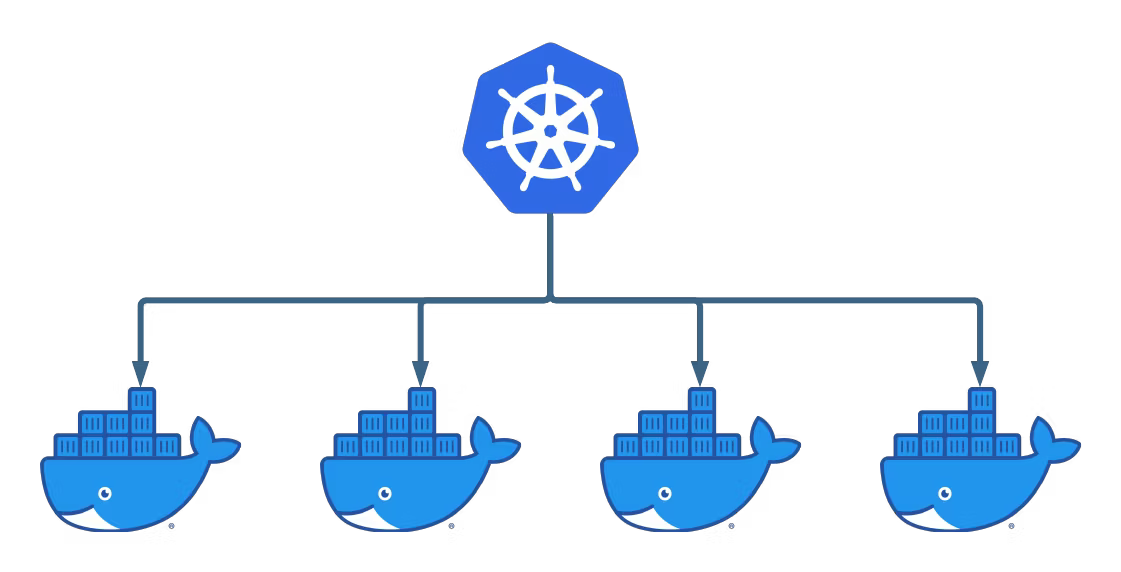
\includegraphics[width=1\textwidth]{Images/2024-04-10-k8s-vs-docker.png}
  \caption{Kubernetes}
  \label{fig:kubernetes}
\end{figure}

Kubernetes is an open-source container orchestration platform originally developed by Google~\cite{kubernetes-docs} 
and now maintained by the Cloud Native Computing Foundation (CNCF)~\cite{cncf-kubernetes}. It automates the deployment, 
scaling, and management of containerized applications across a cluster of machines. Kubernetes abstracts the infrastructure 
and provides primitives such as Pods, Deployments, Services, and Jobs, which allow developers to define complex systems 
declaratively.

% TODO more

In this project, Kubernetes serves as the core infrastructure layer for deploying isolated environments, managing job execution, 
and ensuring scalability and fault tolerance. The native support for namespaces, role-based access control (RBAC), and persistent 
volumes (PVs) makes it suitable for building multi-user platforms.
\section{Microservices}

The microservices architectural style structures an application as a collection of loosely coupled services, each responsible for 
a specific domain or capability~\cite{newman-microservices}. Microservices communicate primarily through lightweight mechanisms 
such as HTTP or messaging queues, and they are independently deployable.

This approach was adopted in the system to improve modularity and separation of concerns. For instance, authentication, job 
orchestration, and storage abstraction are implemented as separate services, allowing them to evolve independently and scale 
according to their individual loads.

\begin{figure}[h!]
  \centering
  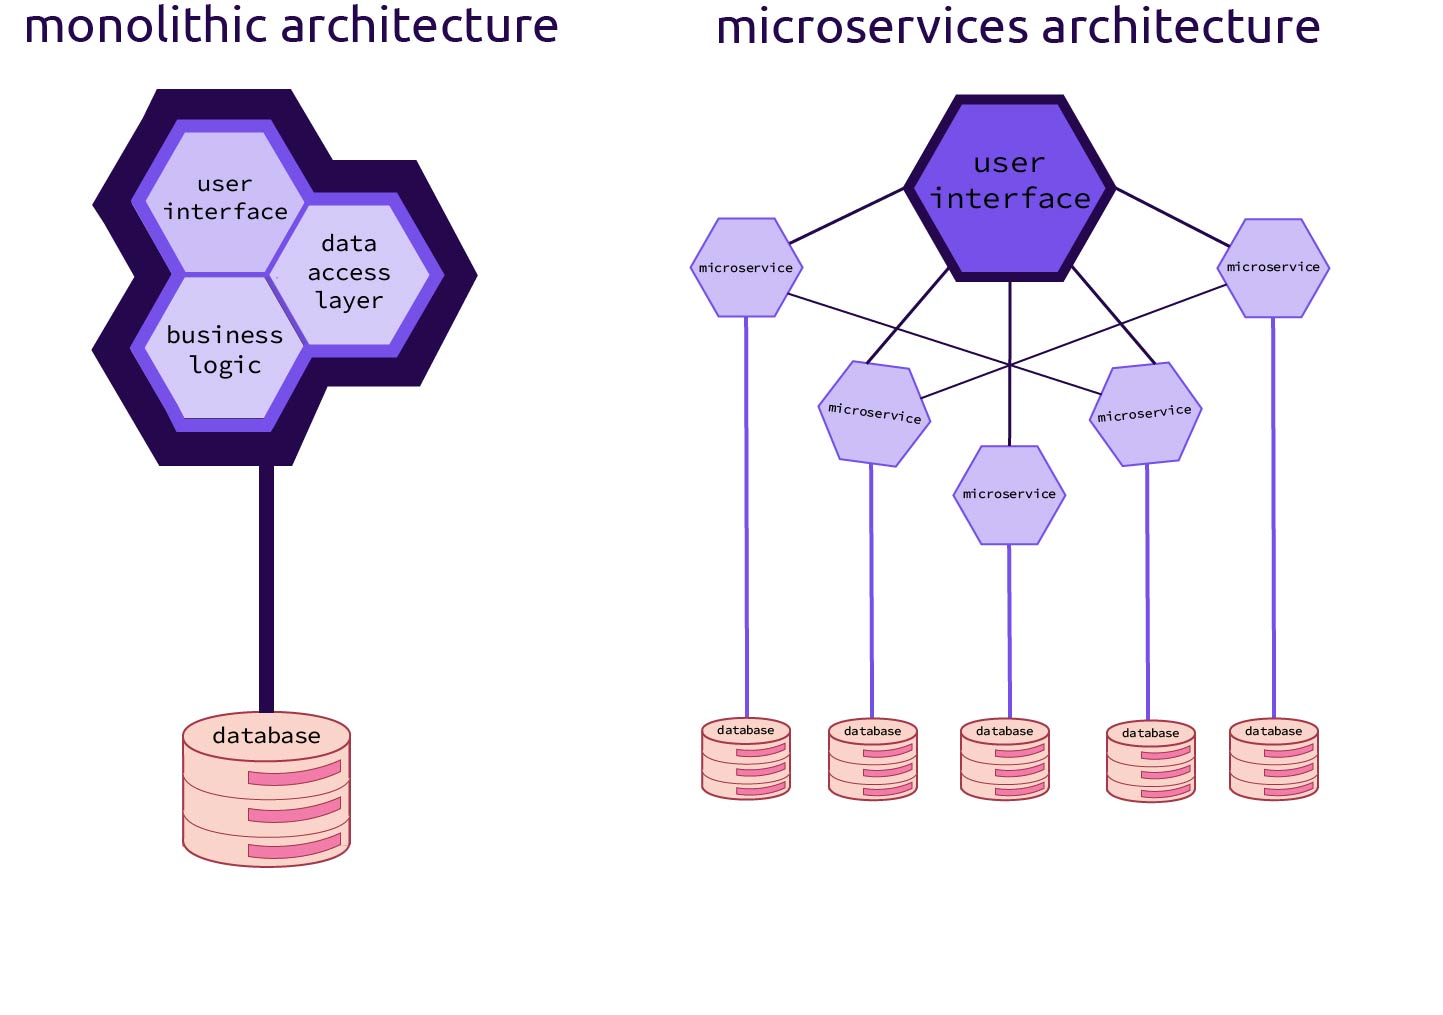
\includegraphics[width=1\textwidth]{Images/monoliths-vs-microservices-whats-the-difference_2.png}
  \caption{MicroServices vs Monolithic}
  \label{fig:microservicesVmonolithic}
\end{figure}

\section{Batch Job Execution}

Batch processing refers to the execution of non-interactive, background jobs that process data in large volumes~\cite{batch-processing}. 
Unlike real-time systems, batch jobs are scheduled and executed at specified times or on demand, often in isolated environments.

Kubernetes natively supports batch job execution through the \texttt{Job} and \texttt{CronJob} resources. In the designed system, 
batch jobs are launched on behalf of users to run data analysis scripts using containerized tools like DuckDB or Pandas, with each 
job being tracked and managed independently.

\section{MinIO}

\begin{figure}[h!]
  \centering
  
\includegraphics[width=0.5\textwidth]{Images/minIO.png}
  \caption{MinIO}
  \label{fig:minio}
\end{figure}

MinIO is a high-performance, Kubernetes-native object storage system compatible with the Amazon S3 API~\cite{minio-docs}. 
It is often used in cloud-native applications to store unstructured data such as logs, images, or datasets.

In the system, MinIO acts as the backend storage for user-uploaded files and job outputs. Its compatibility with S3 allows for flexible 
integration with analytics tools and easy management of large datasets without a traditional POSIX filesystem. 

Additionally, the imaged application tools used in the system are set with I/O on MinIO.
\section{DuckDB}

DuckDB is an in-process SQL OLAP (Online Analytical Processing) database management system optimized for analytical queries on 
columnar data~\cite{duckdb-paper}. Unlike traditional database servers, DuckDB runs directly within the host process and is designed for interactive 
analytics on local files such as CSV and Parquet. Its columnar storage model and vectorized query execution engine make it particularly 
suitable for analytical workloads involving large datasets.

DuckDB draws conceptual inspiration from systems like PostgreSQL and MonetDB, but emphasizes lightweight deployment and embeddability. 
It supports complex SQL queries, window functions, joins, and aggregations with high performance, while avoiding the operational 
complexity of client-server architectures.

\subsection*{Why DuckDB?}

\begin{figure}[h!]
  \centering
  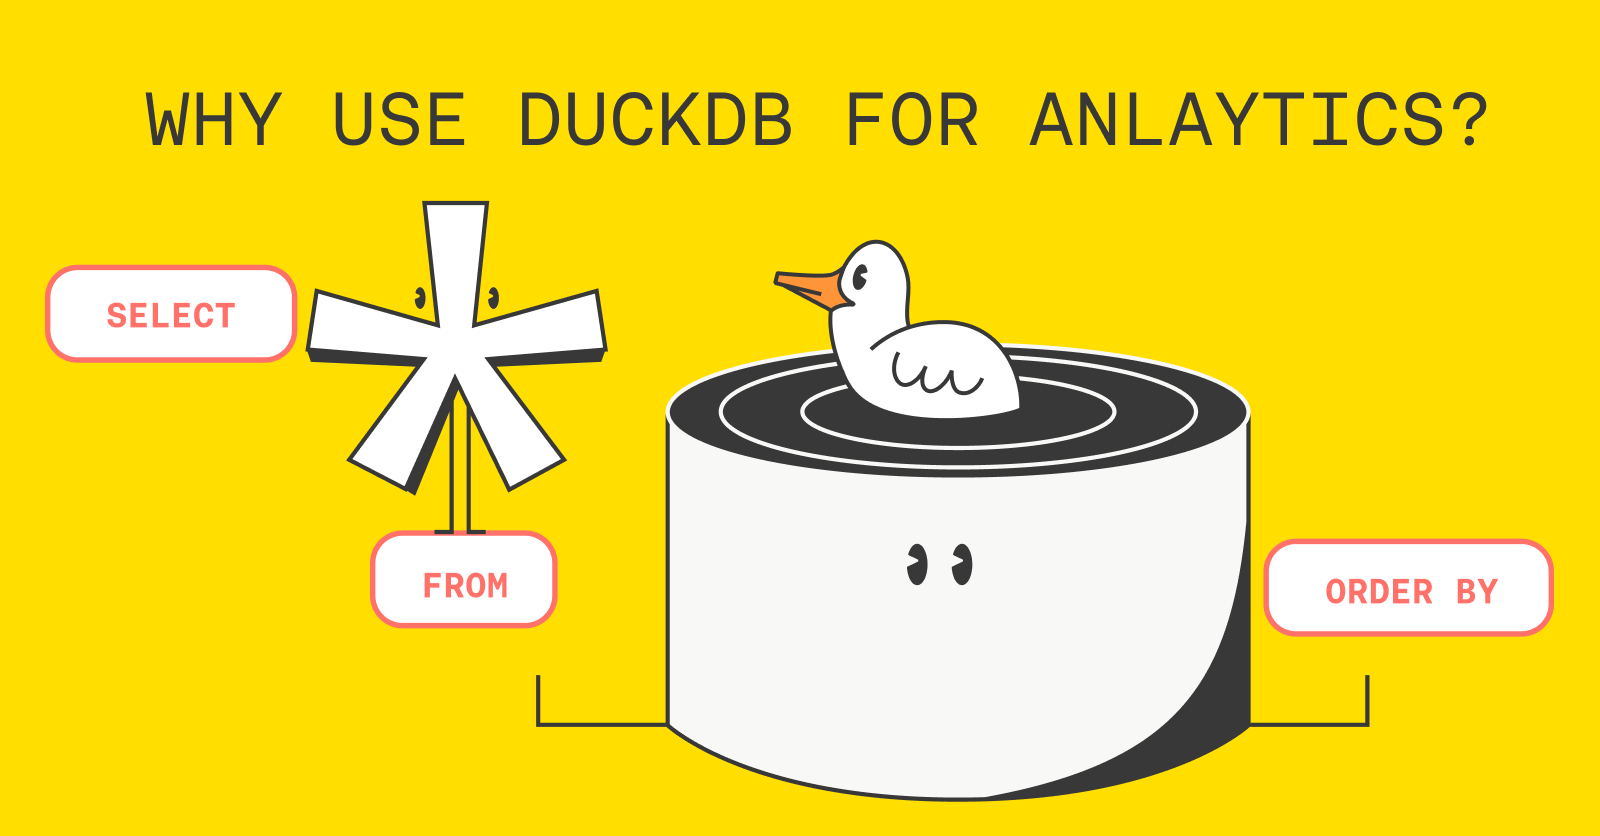
\includegraphics[width=1\textwidth]{Images/duckdb_for_analytics_1_c16a0acfc3.png}
  \caption{Why DuckDB}
  \label{fig:duckdb}
\end{figure}

DuckDB was chosen for this system due to several compelling advantages:

\begin{itemize}
    \item \textbf{Embeddability:} DuckDB can be run inside a container with no setup or external dependencies, making it ideal for 
    sandboxed job execution in Kubernetes.
    
    \item \textbf{Zero Configuration:} Users can query structured files (e.g., CSV, Parquet) without needing to first load data 
    into database tables, simplifying the user workflow.
    
    \item \textbf{Columnar Execution:} Optimized for analytical queries, DuckDB's columnar execution model enables efficient 
    processing of large datasets, particularly in filtering and aggregation operations.
    
    \item \textbf{File-Native Access:} Direct support for querying local data files stored on persistent volumes or object 
    storage simplifies integration with the storage layer (MinIO).
    
    \item \textbf{Lightweight and Fast:} Compared to heavier analytical engines, DuckDB has a small footprint and fast startup time, 
    which makes it suitable for short-lived Kubernetes jobs.
\end{itemize}

In this system, DuckDB is one of the containerized tools available for users to execute SQL-based data analysis jobs on uploaded datasets. 
Its integration enables users to perform complex transformations and analytics directly on their data without managing database 
infrastructure.

\section{SQLite}

\begin{figure}[h!]
  \centering
  
\includegraphics[width=0.5\textwidth]{Images/sqlite-chatgpt-img.png}
  \caption{SQLite}
  \label{fig:sqlite}
\end{figure}

SQLite is a lightweight, serverless, self-contained SQL database engine~\cite{sqlite-docs}. Unlike traditional client-server databases, 
SQLite operates directly on a single disk file and does not require a separate database server process. Its simplicity, low resource 
overhead, and zero-configuration nature make it an ideal choice for embedded applications and local data persistence.

In this system, SQLite is used as the backend storage mechanism for several services, including authentication (Minioth), 
filesystem metadata (Fslite), and job tracking (Uspace). Each service maintains its own isolated SQLite instance, ensuring 
modularity and local data consistency. The relational model of SQLite provides a robust framework for enforcing constraints, 
indexing, and transactional integrity, all while maintaining high performance for low- to moderate-volume workloads.

Due to its embeddable nature, SQLite enables rapid development and deployment of microservices without the overhead of managing 
a centralized database server. This aligns well with the platform’s goals of simplicity, portability, and lightweight infrastructure.


\section{WebSockets}
\begin{figure}[h!]
  \centering
  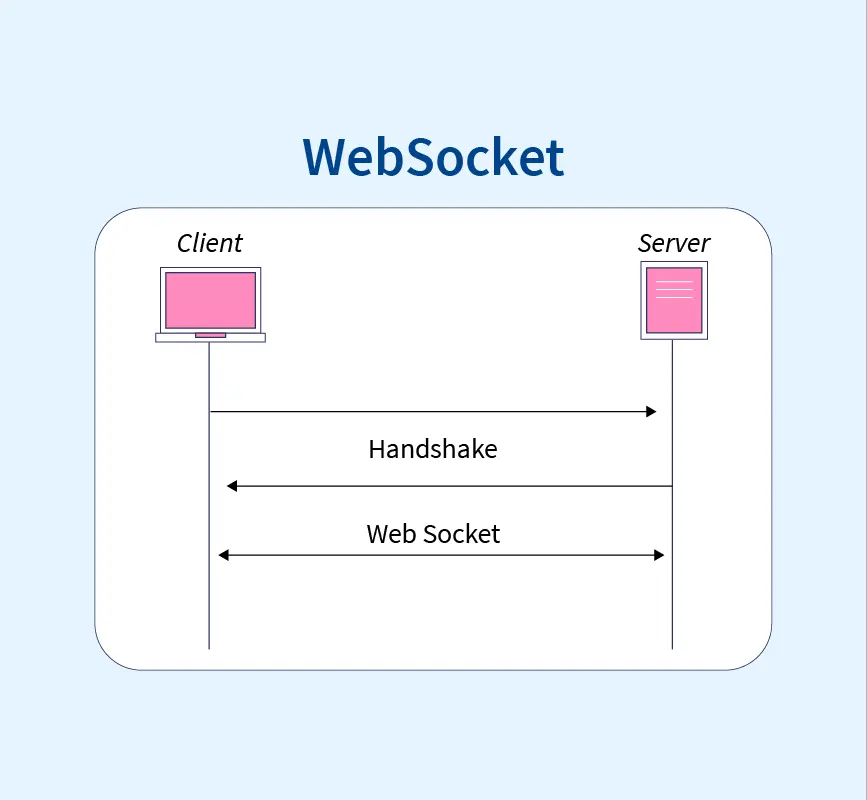
\includegraphics[width=0.8\textwidth]{Images/websockets-1.png}
  \caption{WebSockets}
  \label{fig:websockets}
\end{figure}

WebSockets provide a full-duplex communication channel over a single TCP connection, allowing real-time interaction between 
clients and servers~\cite{ietf-websocket}. Unlike traditional HTTP, WebSockets maintain a persistent connection, enabling low-latency communication.

The system utilizes WebSockets to allow users to interact with their environment in real time, including job monitoring and 
event-driven communication with backend services.
\section{Containers}

\begin{figure}[h!]
  \centering
  
\includegraphics[width=0.5\textwidth]{Images/what-is-docker.png}
  \caption{Docker Containers}
  \label{fig:docker-containers}
\end{figure}

Containers are lightweight, portable units that package software with its dependencies and run isolated from the host 
system~\cite{docker-docs}. Technologies like Docker and container runtimes such as containerd have made containers a 
standard deployment model in modern systems.

In this system, each analytical job is executed within its own container, ensuring environment reproducibility and isolation 
between users. This also facilitates the inclusion of tools like Bash, Octave, and Python in a controlled, sandboxed manner.

The Microservices theirselves will be deployed as individual containers in collaboration with K8S.
\section{Multi-User System Design}

A multi-user system is one that supports concurrent access by multiple independent users, often with varying levels of access, 
permissions, and isolation. In such systems, key design considerations include authentication, authorization, resource sharing, 
and conflict avoidance~\cite{tanenbaum-os}.

The platform presented in this thesis implements a multi-user architecture where each user is assigned a secure, isolated environment. 
Users may upload datasets, execute jobs, and share resources depending on their group memberships and permissions. This design is 
inspired by UNIX-like models, incorporating user/group-based access control to enforce data protection and operational boundaries 
within a shared infrastructure.

\newpage
\section{Authentication Model}

Authentication is the process of verifying the identity of users before granting access to system resources~\cite{ferraiolo-auth}. 
In multi-user systems, secure and reliable authentication is foundational to ensuring that only authorized users can interact with 
sensitive data or operations.

The system utilizes a custom-built authentication service called \texttt{Minioth}, which follows a token-based authentication scheme 
using JSON Web Tokens (JWT). Upon successful login, users receive short-lived signed tokens that are used to authenticate future requests. 
This stateless approach enables efficient, scalable identity verification across distributed microservices, while also supporting user and 
group management for access control.

\newpage
\section{Cloud-Native Storage}

\begin{figure}[h!]
  \centering
  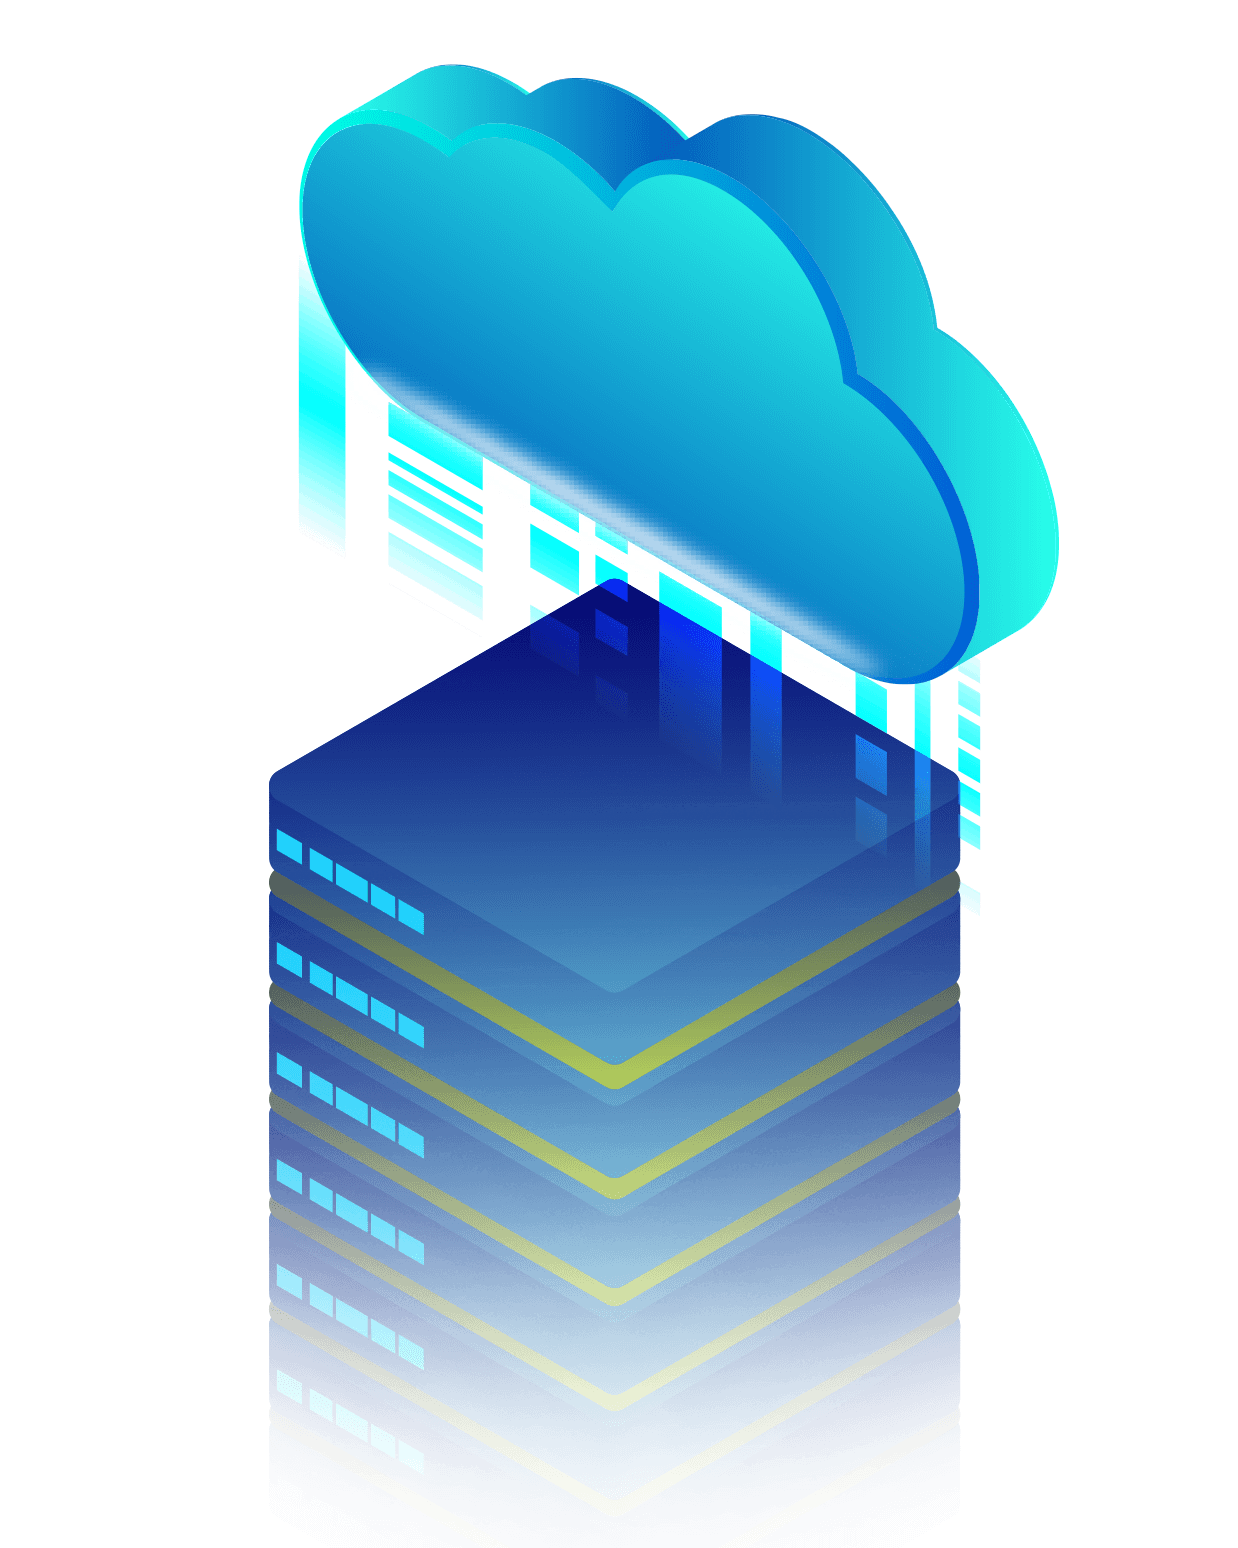
\includegraphics[width=0.4\textwidth]{Images/img-hybrid-cloud-engineer.png}
  \caption{CNS}
  \label{fig:cns}
\end{figure}

Cloud-native storage refers to storage systems designed to operate within cloud environments, typically containerized and orchestrated 
via platforms like Kubernetes~\cite{cncf-storage}. Unlike traditional block or file-based storage, cloud-native storage solutions are 
optimized for dynamic workloads, scalability, and high availability.

In this system, MinIO—a cloud-native object storage service compatible with Amazon S3—is used to store user data and job outputs. 
Object storage offers flexibility in managing large, unstructured datasets, and integrates seamlessly with Kubernetes via 
Persistent Volume Claims (PVCs). Cloud-native storage allows the system to dynamically provision isolated storage volumes for each 
user or job, supporting scalable and fault-tolerant operations.


\chapter{Related Work}
\label{Chapter-Related-Work}

% Todo: Edit to your liking
\section{Related work A}
\section{Related work B}

\section{The FPGA Perspective}
\section{Thesis Approach}

\chapter{Robustness Analysis}
\label{Chapter-Robustness-Analysis}

% Todo: Edit to your liking
\section{Experiment A}
\section{Experiment B}

\chapter{Results}
\label{Chapter-Results}

\section{Specification of Compared Platforms}
\section{Power Consumption}
\section{Energy Consumption}
\section{Throughput and Latency Speedup}
\section{Final Performance}

\chapter{Conclusions and Future Work}
\label{Chapter-Conclusions-and-Future-Work}

\section{Conclusions}
\section{Future Work}


%----------------------------------------------------------------------------------------
%	THESIS CONTENT - APPENDICES
%----------------------------------------------------------------------------------------

\appendix % Cue to tell LaTeX that the following "chapters" are Appendices

% Include the appendices of the thesis as separate files from the Appendices folder
% Uncomment the lines as you write the Appendices

% Todo: comment out if not needed
% Appendix A

\chapter{Frequently Asked Questions} % Main appendix title

\label{AppendixA} % For referencing this appendix elsewhere, use \ref{AppendixA}

\section{How do I change the colors of links?}

The color of links can be changed to your liking using:

{\small\verb!\hypersetup{urlcolor=red}!}, or

{\small\verb!\hypersetup{citecolor=green}!}, or

{\small\verb!\hypersetup{allcolor=blue}!}.

\noindent If you want to completely hide the links, you can use:

{\small\verb!\hypersetup{allcolors=.}!}, or even better: 

{\small\verb!\hypersetup{hidelinks}!}.

\noindent If you want to have obvious links in the PDF but not the printed text, use:

{\small\verb!\hypersetup{colorlinks=false}!}.

% \chapter*{Appendix: Source Code Access}
The full source code of the project, including the backend services, FrontApp UI, and deployment configurations, can be found at:

\url{https://github.com/kyri56xcaesar/kuspace}

% \include{Appendices/AppendixC}

%----------------------------------------------------------------------------------------
%	BIBLIOGRAPHY
%----------------------------------------------------------------------------------------

\cleardoublepage\phantomsection\addcontentsline{toc}{chapter}{References}
\printbibliography[keyword={References}, title={References}]
\printbibliography[keyword={Link}, title={External Links}]

%----------------------------------------------------------------------------------------

\end{document}